\chapter{Results and Evaluation} \label{chap:result}
{\color{red}Give some introduction, the structure of this chapter.}

\textbf{Parameter setup}
First we need to specify the parameters we used throughout the whole evaluation part. 
The default parameters are applied for the RGBD-Fusion method, which has 8 in total. 
It should be mentioned that, since both proposed methods don't have smoothness term for the depth enhancement, the $\lambda_z^2$ in RGBD-Fusion and $\lambda_l$ in our implementation RGBD-Fusion Like method are set to 0 for the sake of fairness comparison.
Only during the quantitative evalution, we want to illustrate the importance of this smoothness term so the $\lambda_z^2$ and $\lambda_l$ are set to the values in table~\ref{tab:parameter_setup}.

\begin{table}[!ht]
\caption{Parameters of all the methods throughout all the experiments.}
\label{tab:parameter_setup}
\centering
\begin{tabular}{|m{4cm} |m{1.5cm} |m{7cm}|}
\hline
Method                               & \multicolumn{1}{c|}{Total number} & \multicolumn{1}{c|}{Parameters}                                                                                                                                          \\ \hline
RGBD-Fusion~\cite{or2015rgbd} & \multicolumn{1}{c|}{8}            &{$\lambda_\rho = 0.1, \lambda_\beta^1 = 0.1, \lambda_\beta^2 = 0.1, \tau = 0.05, \sigma_c = \sqrt{0.05}, \sigma_d = \sqrt{50}, \lambda_z^1 = 0.004, \lambda_z^2 = 0.0075$} \\ \hline
RGBD-Fusion Like                    & \multicolumn{1}{c|}{5}             & {$\lambda_{\rho} = 10, \sigma_I = \sqrt{0.05}, \sigma_z = \sqrt{50}, \lambda_z = 500, \lambda_l = 2$}                                                                                                                                                                         \\ \hline
Proposed I: RGB Ratio                            & \multicolumn{1}{c|}{4}             & $\lambda_{\rho}^1 = 10^{15}, \lambda_{\rho}^2 = 10^{13}, \sigma_c = 100, \lambda_z = 100$                                                                                                                                                                                                                                                                                                                                                  \\ \hline
Proposed II: Multi-Light                          & \multicolumn{1}{c|}{1}            & $\lambda_z = 100$                                                                                                                                                                          \\ \hline
\end{tabular}
\end{table}


%%%%%%%%%%%%%%%%%%%%%%%%%%%%%%%%%%%%%%%%%%%%
\section{Quantitative Evaluation}
%%%%%%%%%%%%%%%%%%%%%%%%%%%%%%%%%%%%%%%%%%%%
\textbf{Data generation}
In order to quantitatively validate the performance of our proposed methods and our implementation of the RGBD-Fusion, we use the well-known "The Joyful Yell" dataset with 3 point light sources and ambient lights. 
Three various albedo scenarios are considered: 
\begin{itemize}
    \item Red, green and blue piece-wise constant areas
    \item Colorful patterns with a few small details inside\footnote{EBSD map. Image Courtesy of \url{https://mtex-toolbox.github.io/files/doc/EBSDSpatialPlots.html}}
    \item Colorful patterns with complicated details\footnote{1000 Visual Mashups. Image Courtsesy of \url{https://www.flickr.com/photos/qthomasbower/3470650293}}
\end{itemize}


To simulate the natural scene illumination, we assume the RGB lighting as frontal directions, so the first-order SH parameters are modelled as:
\begin{equation*}
    \mathbf{s}_R = \mathbf{s}_G = \mathbf{s}_B = \begin{bmatrix} 0 & 0& -1 & 0.2\end{bmatrix}^\top
    \qquad
    \raisebox{-0.7cm}{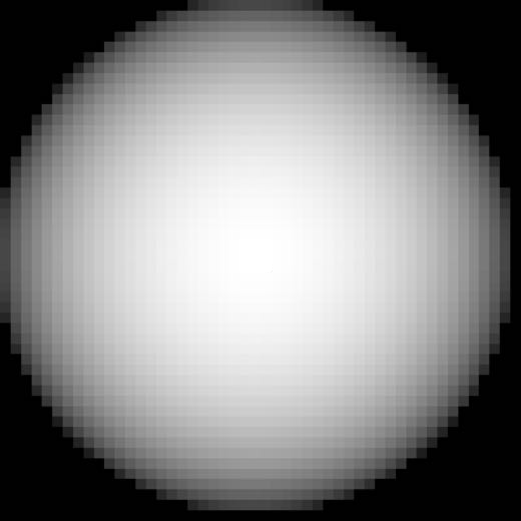
\includegraphics[height=0.1\textwidth]{figures/result/light9.pdf}}
\end{equation*}

And then, in order to reproduce the LED configuration for the proposed RGB ratio model, we define the 3 lighting directions as:
\begin{equation*}
    \begin{split}
        \mathbf{s}_R &= \begin{bmatrix} 0 &0 &-1 &0.15\end{bmatrix}^\top\\
        \mathbf{s}_G &= \begin{bmatrix} 0.3 & 0.2 & -1 & 0.25\end{bmatrix}^\top\\
        \mathbf{s}_B &= \begin{bmatrix} -0.2 & 0.3 & -1 & 0.2\end{bmatrix}^\top\\
    \end{split}
    \qquad\qquad\quad
    \raisebox{-0.7cm}{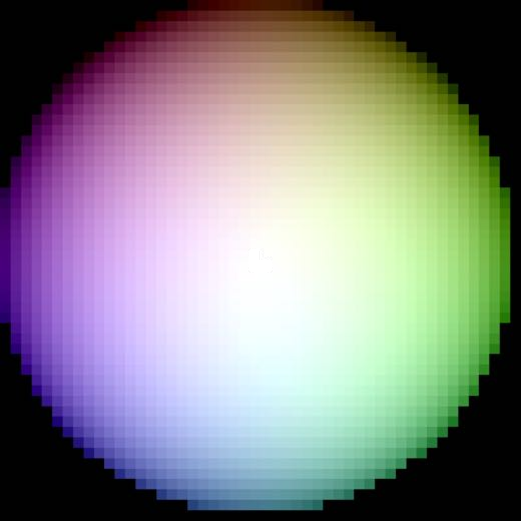
\includegraphics[height=0.1\textwidth]{figures/result/light_color.pdf}}
\end{equation*}
Finally, we need to produce a sequence of same images with various directional lights for our robust multi-light model.
A "lighting" matrix $L$ and the corresponding positions of 10 point light sources can be illustrated as below, where red points represent the light positions.
\begin{equation*}
\begin{split}
L = 
    \begin{pmatrix}
        0.5 & 0 & -1 & 0.2\\
        0.3 & 0.4 & -1 & 0.2\\
        0 & 0.5 & -1 & 0.2\\
        -0.4 & 0.3 & -1 & 0.2\\
        -0.5 & 0 & -1 & 0.2\\
        -0.3 & -0.4 & -1 & 0.2\\
        0 & -0.5 & -1 & 0.2\\
        0.4 & -0.3 & -1 & 0.2\\
        0 & 0 & -1 & 0.2\\
        0.45 & 0.2 & -1 & 0.2\\
    \end{pmatrix}^\top 
    \qquad 
    &\raisebox{-2.8cm}{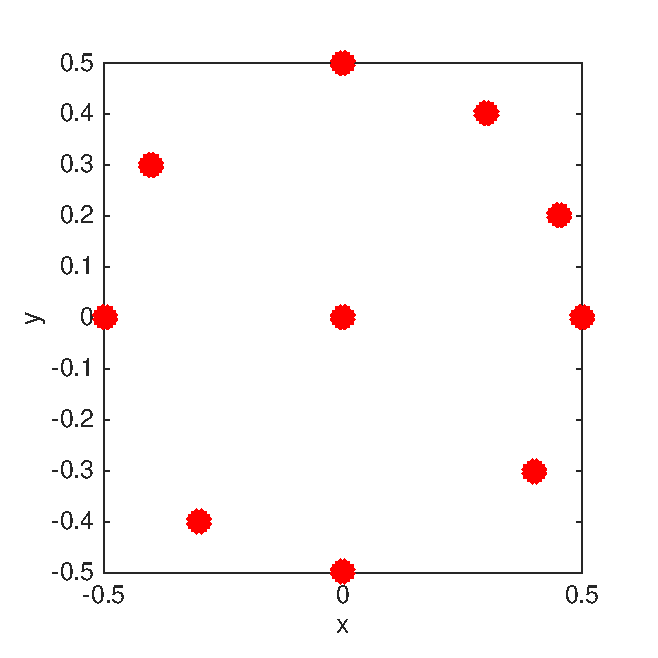
\includegraphics[height=0.4\textwidth]{figures/result/example_multi_light.eps}}\\
    \raisebox{-0.4cm}{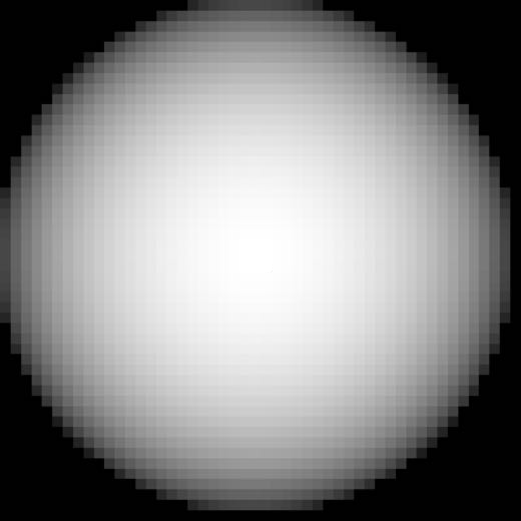
\includegraphics[height=0.1\textwidth]{figures/result/light9.pdf}}    
    \raisebox{-0.4cm}{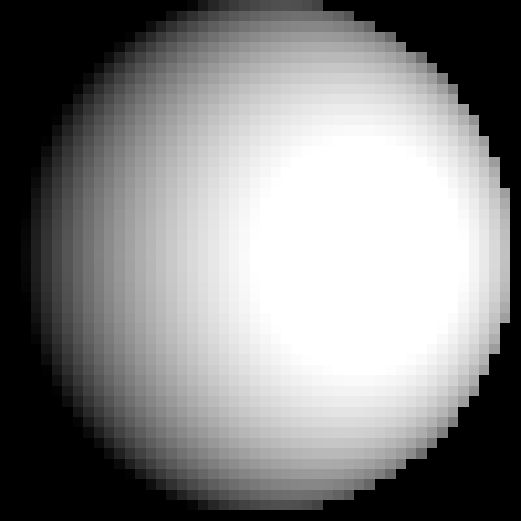
\includegraphics[height=0.1\textwidth]{figures/result/light1.pdf}}
    \raisebox{-0.4cm}{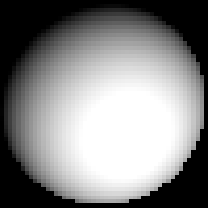
\includegraphics[height=0.1\textwidth]{figures/result/light2.pdf}}
    \raisebox{-0.4cm}{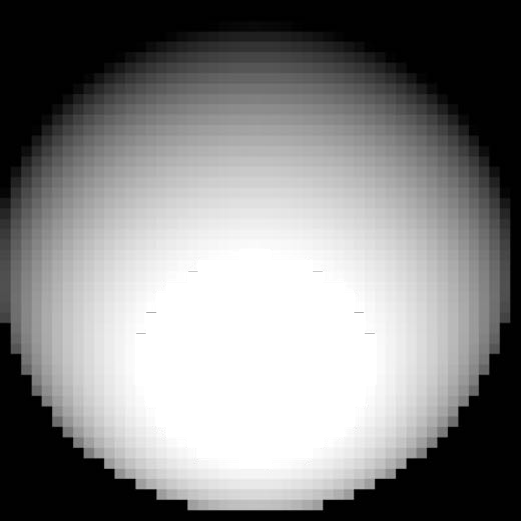
\includegraphics[height=0.1\textwidth]{figures/result/light3.pdf}}
    \raisebox{-0.4cm}{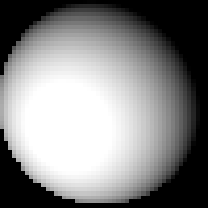
\includegraphics[height=0.1\textwidth]{figures/result/light4.pdf}}
    &\raisebox{-0.4cm}{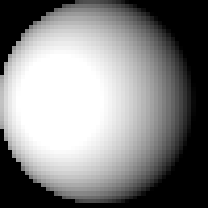
\includegraphics[height=0.1\textwidth]{figures/result/light5.pdf}}
    \raisebox{-0.4cm}{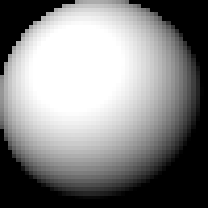
\includegraphics[height=0.1\textwidth]{figures/result/light6.pdf}}
    \raisebox{-0.4cm}{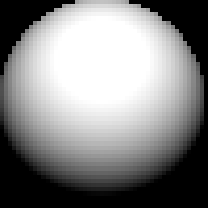
\includegraphics[height=0.1\textwidth]{figures/result/light7.pdf}}
    \raisebox{-0.4cm}{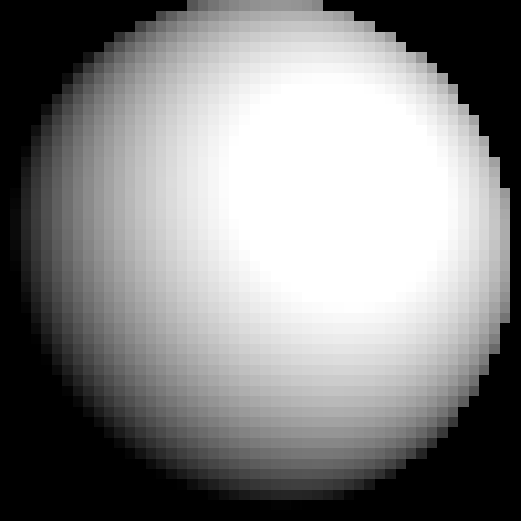
\includegraphics[height=0.1\textwidth]{figures/result/light8.pdf}}
    \raisebox{-0.4cm}{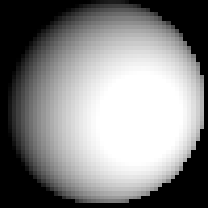
\includegraphics[height=0.1\textwidth]{figures/result/light10.pdf}}
    \end{split}
\end{equation*}

With the 3 different albedos and all the pre-defined lights, we can create the synthetic color images like the first row in Fig.~\ref{fig:result_syn_comp}.

\textbf{Metrics}
Two metrics have been defined to quantitatively evaluate the performance of depth refinement: root mean square error (RMSE) and mean angular error (MAE).
Since we have already had the input rough depth and the ground truth depth as shown in Fig.~\ref{fig:comp_syn_input}, we can define two metrics as follows.

Assuming $z_g, N_g$ and $z, N$ are the ground truth and the refined depth and normal respectively, $m$ the total number of pixels inside the given mask $\mathcal{M}$ and $i$ the index inside the mask, a loosely definition is: 
\begin{align}
    e_{RMSE} &= \sqrt{\frac{\sum\limits_{i}^{m}{(z(i) - z_g(i))^2}}{m}}\\
    e_{MAE} &= \frac{\sum\limits_{i}^{m} \arccos (N(i) \cdot N_g(i))}{m}
\end{align}
The RMSE reflects refined depth quality, while the MAE illustrates if the refined object's shape is similar to the real one. 
It should be mentioned that $e_{MAE}$ gives values in radians but we convert it to degrees.

\begin{table}[!ht]
\caption{Quantitative evaluations among 4 methods. RMSE and MAE are in pixels and degrees respectively. "No smooth" means no laplacian smoothness term in depth enhancement.}
\vspace{1em}
\label{tab:comp_syn_eval}
\centering
\begin{tabular}{lllllll}
                                       & \multicolumn{2}{c}{Simple RGB}                     & \multicolumn{2}{c}{Pattern}                        & \multicolumn{2}{c}{Complicated Pattern}            \\\hline
Method                                 & \multicolumn{1}{c}{RMSE} & \multicolumn{1}{c}{MAE} & \multicolumn{1}{c}{RMSE} & \multicolumn{1}{c}{MAE} & \multicolumn{1}{c}{RMSE} & \multicolumn{1}{c}{MAE} \\\hline\hline
Input reference                              & 3.3305                   & 16.3096                 & 3.3305                   & 16.3096                 & 3.3305                   & 16.3096                 \\
RGBD-Fusion\cite{or2015rgbd} (no smooth)                       & 3.3418                   & 18.9115                 & 3.3872                   & 27.0026                 & 3.3411                   & 25.6574  		\\
RGBD-Fusion\cite{or2015rgbd} & 3.1751                   & 17.2197                 & 3.1890                   & 18.4722                 & 3.1708                   & 18.0850                 \\ 
Fusion-Like (no smooth)                  & 3.3475                   & 17.5911                 & 3.3459                   & 23.4808                 & 3.3898                   & 35.2610                 \\
Fusion-Like                        & 2.8700                   & 17.1776                 & 2.8749                   & 17.7302                 & 2.8848                   & 19.6452                 \\
RGB ratio model                        & \textbf{1.9437}          & \textbf{5.0574}         & 2.9116                   & 17.5238                 & 3.1006                   & 21.2286                 \\
Robust multi-light model               & 3.4025                   & 6.6640                  & \textbf{1.5794}          & \textbf{1.7368}         & \textbf{1.8424}          & \textbf{2.6815}  \\\hline      
\end{tabular}
\end{table}


According to table~\ref{tab:parameter_setup},~\ref{tab:comp_syn_eval} and Fig.~\ref{fig:result_syn_comp}, there are some interesting observations:
\begin{itemize}
    \item Our RGBD-Fusion Like method uses less parameters than RGBD-Fusion~\cite{or2015rgbd} (5 against 8) but achieves almost the same results as the original paper. 
    \item The Laplacian smoothness term in the depth enhancement energy of RGBD-Fusion method has a huge impact on the refined results. In contrast, both our proposed methods have no smoothness term but gives equal or better results.
    \item Single depth image refinement methods (RGBD-Fusion and RGB ratio model) have a chance to acquire satisfying results only when the albedo is elementary with several big color patches. 
    However, they will fail and give even worse in terms of RMSE and MAE when the albedos get complex. 
    Most of the small details on the albedo of "Pattern" and "Complicate Pattern" cannot be acquired, which leads to the wrong depth estimation.
    This is due to the fact that the albedo estimation in these methods highly relies on the regularization terms which prefers piecewise smooth, but this does not meet the condition of most real-world objects.
    \item It can be effortlessly noticed that our robust multi-light method has a strong ability to handle the cases with extremely complicated albedo. 
    Instead of using any regularization for calculating the albedo, extra images with various light directions solve the overfitting problems of albedo and enable the albedo estimation with only the SFS term (Eq.~\ref{eq:robust_albedo_estimate}).
\end{itemize}




\begin{figure}[!ht]
\centering
\subfigure[Input depth]{\label{fig:robust_matrix1}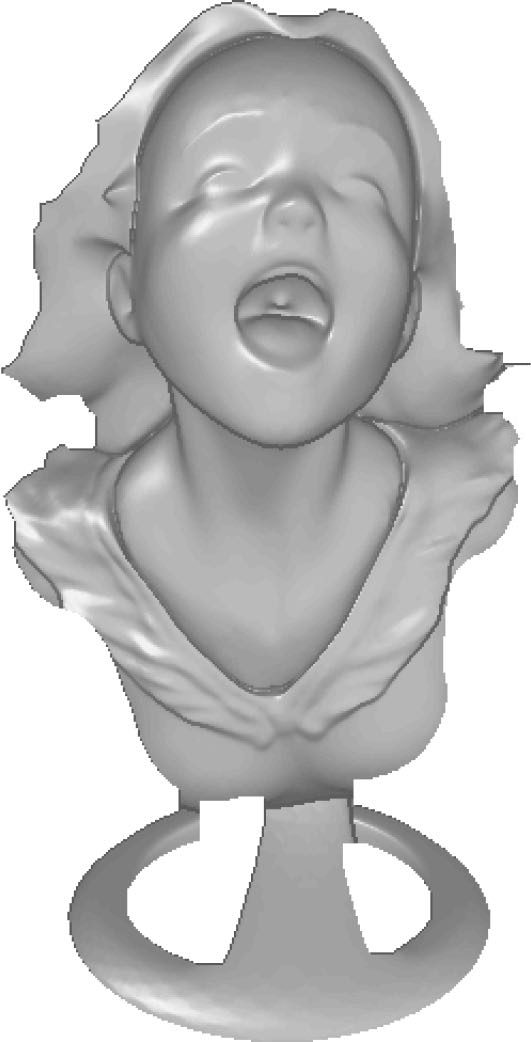
\includegraphics[width=0.2\linewidth]{figures/result/comp_input_shape.pdf}}
\qquad \qquad
\subfigure[Ground truth depth]{\label{fig:robust_matrix2}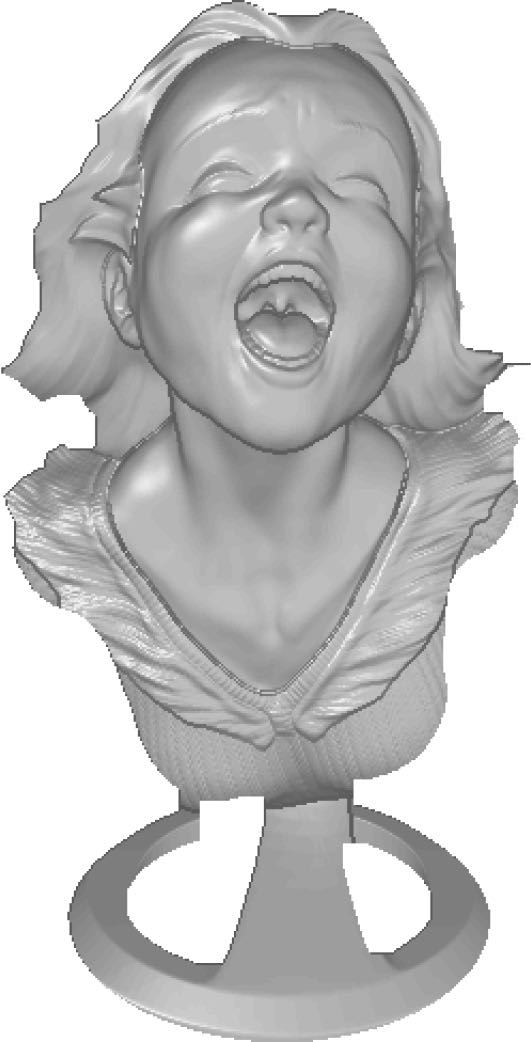
\includegraphics[width=0.2\linewidth]{figures/result/comp_gt_shape.pdf}}
\caption{The 3D shape of input rough depth and the ground truth depth for the quantitative evalution.}
\label{fig:comp_syn_input}
\end{figure}


\begin{figure}
  % Top row: Ground truth, Image + SH, Image + SH, Image + SH
  \setlength{\tabcolsep}{0.5em} % for the horizontal padding
{\renewcommand{\arraystretch}{0.6}% for the vertical padding
\begin{tabular}{cccc}
%    \multicolumn{2}{c}{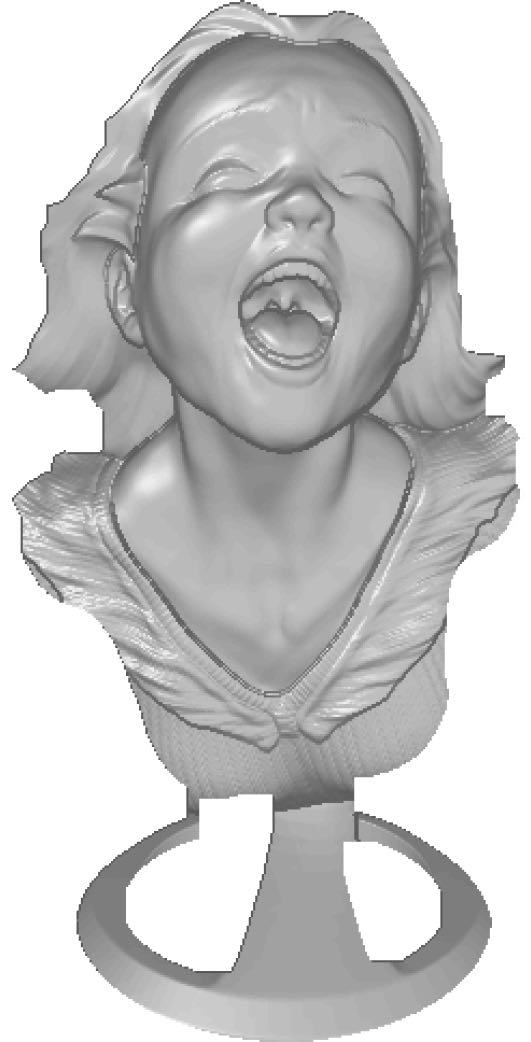
\includegraphics[width=0.1\linewidth]{figures/result/comp_robust_pattern_shape.pdf}} &
&
    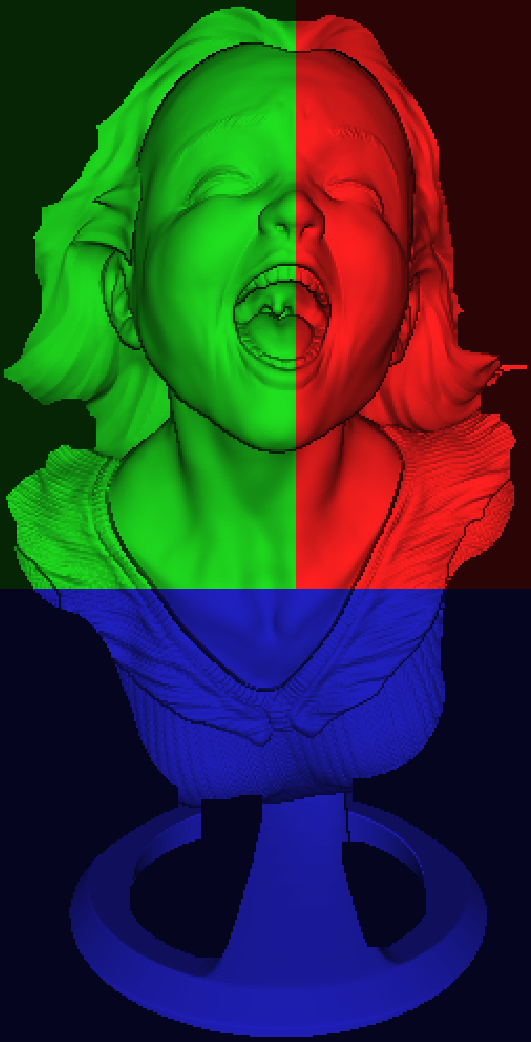
\includegraphics[height=0.25\linewidth]{figures/result/comp_simple_rgb.pdf}
    
\includegraphics[height=0.25\linewidth]{figures/result/comp_simple_albedo.pdf}& 
    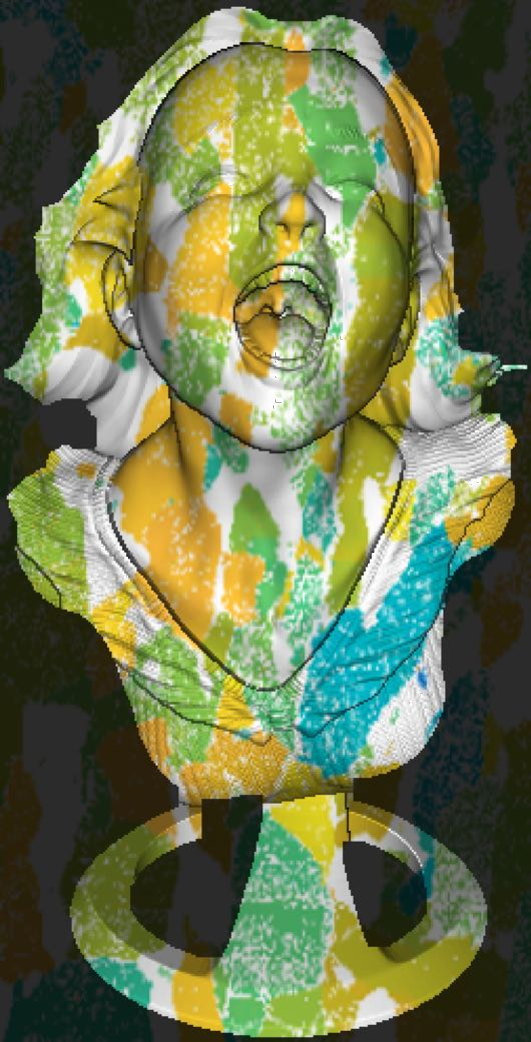
\includegraphics[height=0.25\linewidth]{figures/result/comp_pattern_rgb.pdf} 
    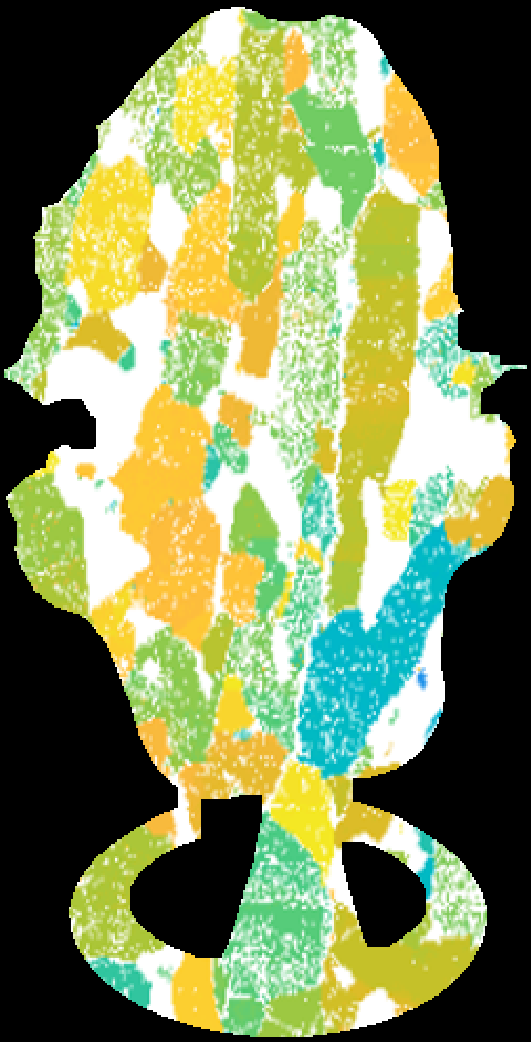
\includegraphics[height=0.25\linewidth]{figures/result/comp_pattern_albedo.pdf}& 
    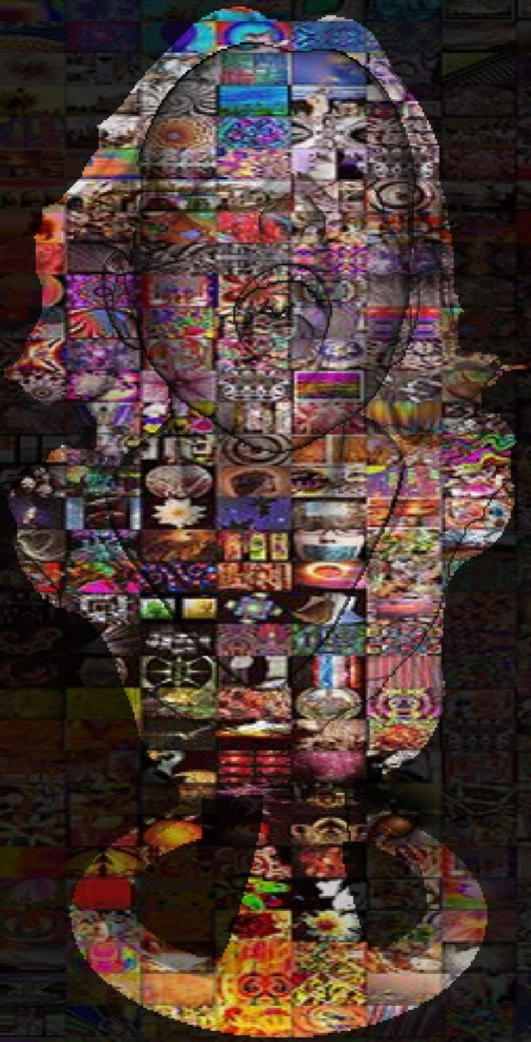
\includegraphics[height=0.25\linewidth]{figures/result/comp_love_rgb.pdf}
    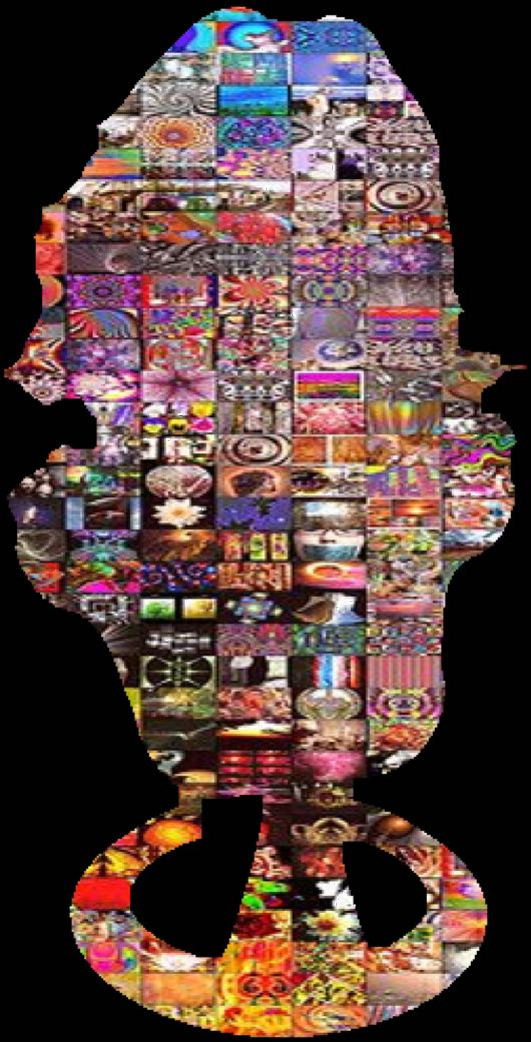
\includegraphics[height=0.25\linewidth]{figures/result/comp_love_albedo.pdf} \\
% \multicolumn{2}{c}{ {\small Ground truth}}  &
     & {\small Simple RGB} & {\small Pattern} & {\small Complicated Pattern } \\
%%%%%%%%%%%%%%%%%%%%%%%%%%%%%%%%%%%%%%%%%%%%%%%%%%%% 
  % Initial guess
  
%  \multirow{2}{*}{
%  \begin{tabular}{c}
%  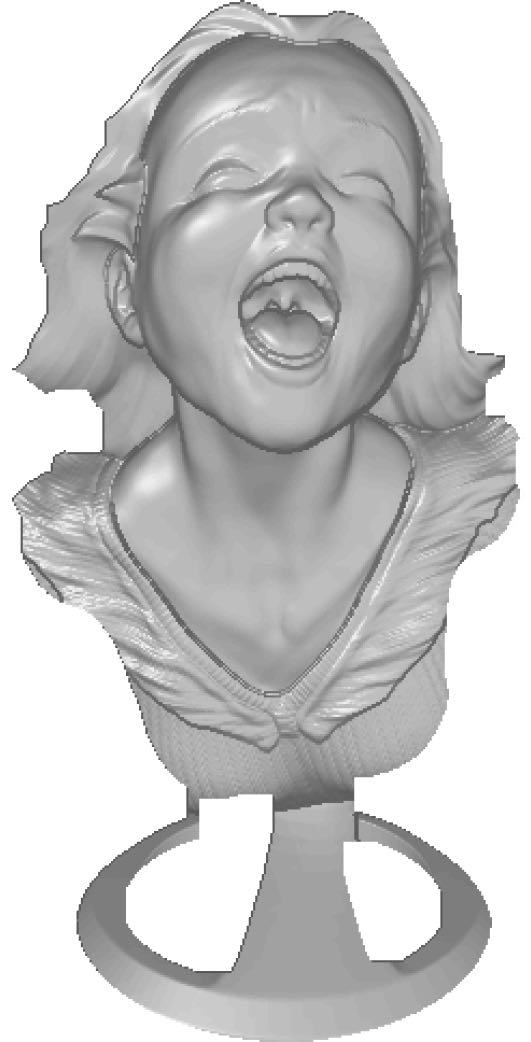
\includegraphics[width=0.1\linewidth]{figures/result/comp_robust_pattern_shape.pdf} \\ Non-realistic \\ initialization 
%  \end{tabular}} &

  % RGBD-Fusion without smoothing
  % Simple RGB
\multirow{-15}{*}{\parbox[t]{2.5mm}{\rotatebox[origin=c]{90}{\small RGBD-Fusion~\cite{or2015rgbd} $\lambda_l = 0$}}} &
 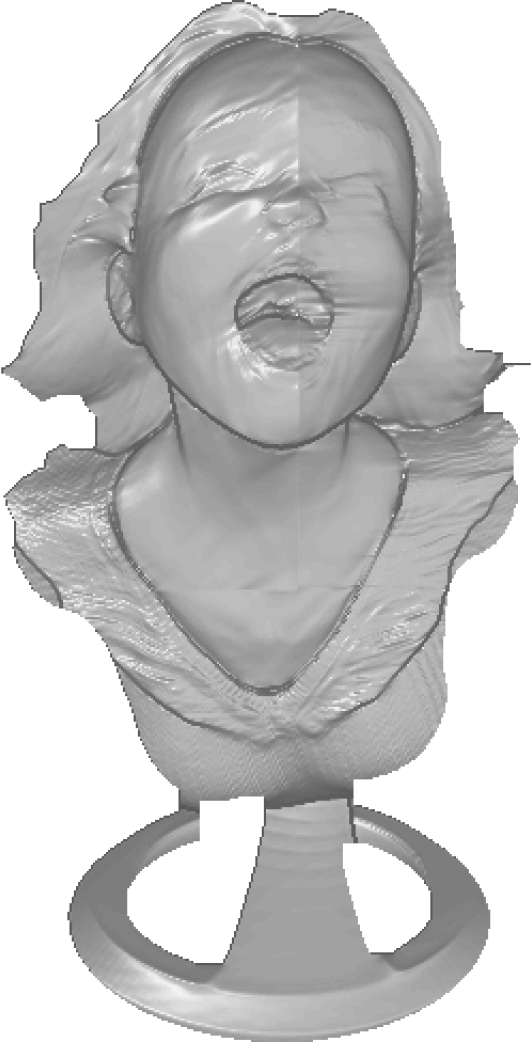
\includegraphics[height=0.25\linewidth]{figures/result/comp_fusion_rgbN_shape.pdf}
 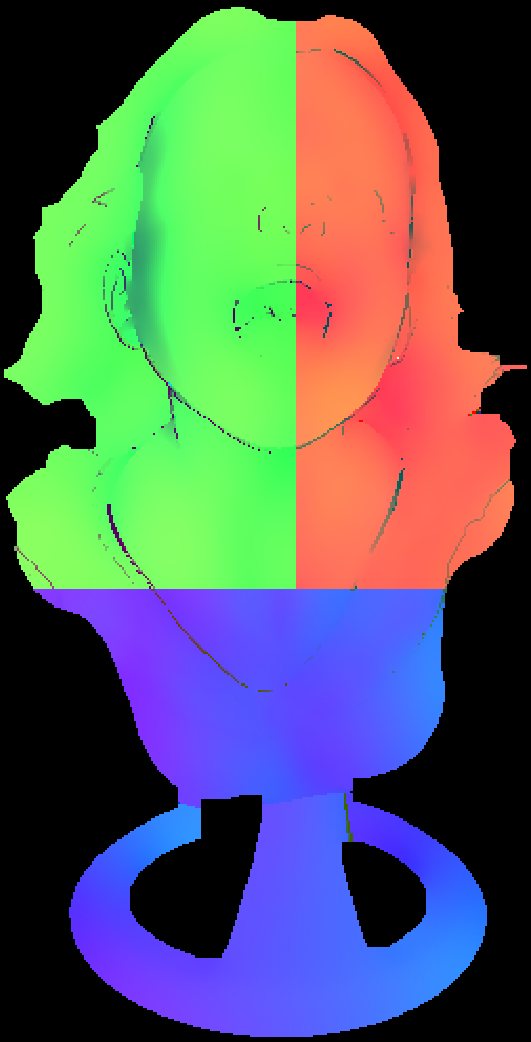
\includegraphics[height=0.25\linewidth]{figures/result/comp_fusion_rgbN_albedo.pdf} &
  % Pattern
 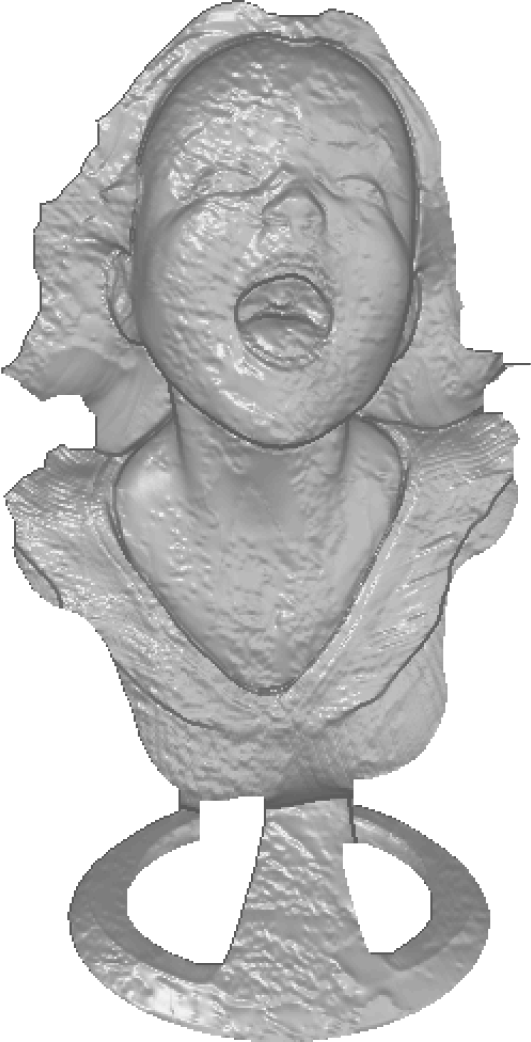
\includegraphics[height=0.25\linewidth]{figures/result/comp_fusion_patternN_shape.pdf} 
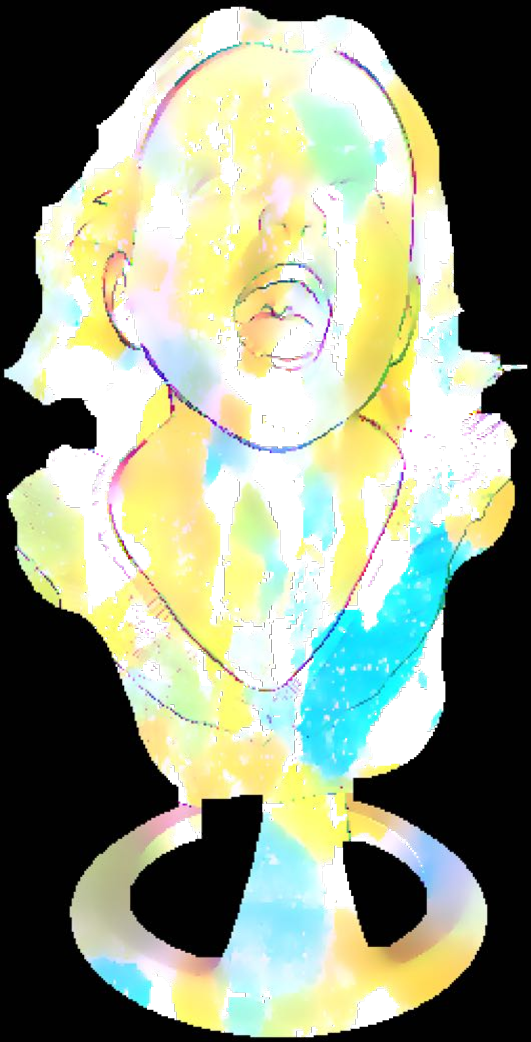
\includegraphics[height=0.25\linewidth]{figures/result/comp_fusion_patternN_albedo.pdf} &
  % Complicate Pattern
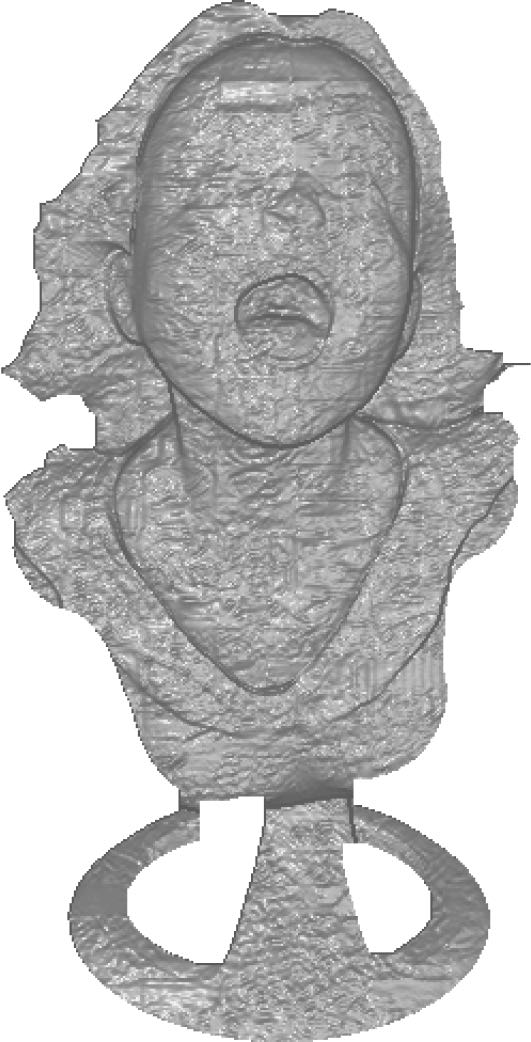
\includegraphics[height=0.25\linewidth]{figures/result/comp_fusion_loveN_shape.pdf} 
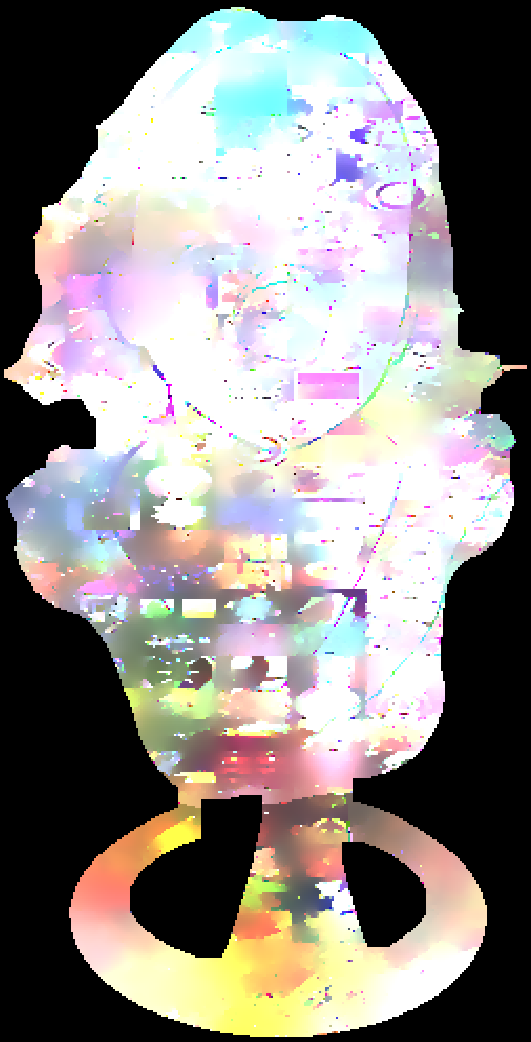
\includegraphics[height=0.25\linewidth]{figures/result/comp_fusion_loveN_albedo.pdf} \\
& {\small RMSE $= 3.35$, MAE $=17.60$} & {\small RMSE $= 3.35$, MAE $=23.48$} & {\small RMSE $= 3.39$, MAE $=35.26$} \\
%%%%%%%%%%%%%%%%%%
  % {\small Non-realistic initial guess} & % Same for SIRFS
  % Ours - Dir
\multirow{-15}{*}{\parbox[t]{2.5mm}{\rotatebox[origin=c]{90}{\small RGBD-Fusion~\cite{or2015rgbd}}}}&
 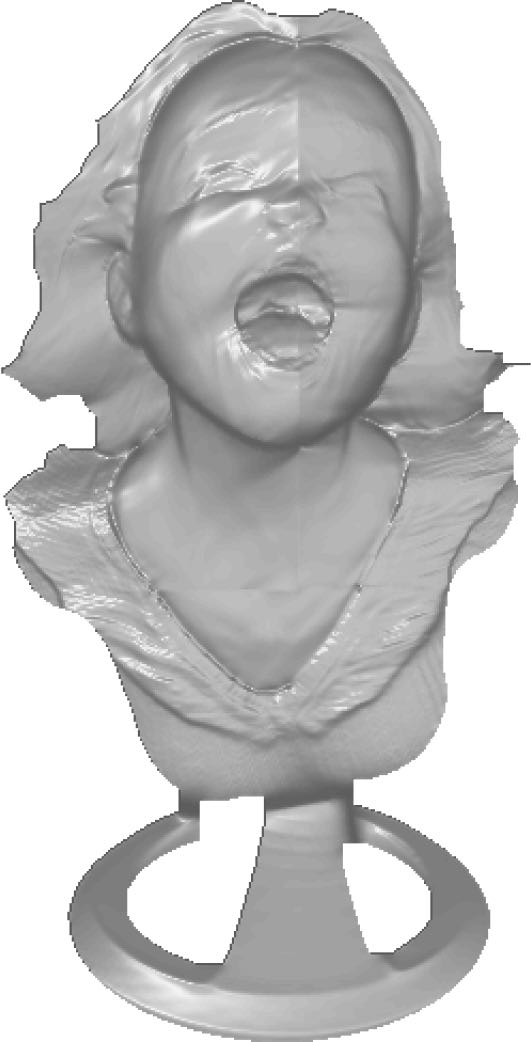
\includegraphics[height=0.25\linewidth]{figures/result/comp_fusion_rgb_shape.pdf}
 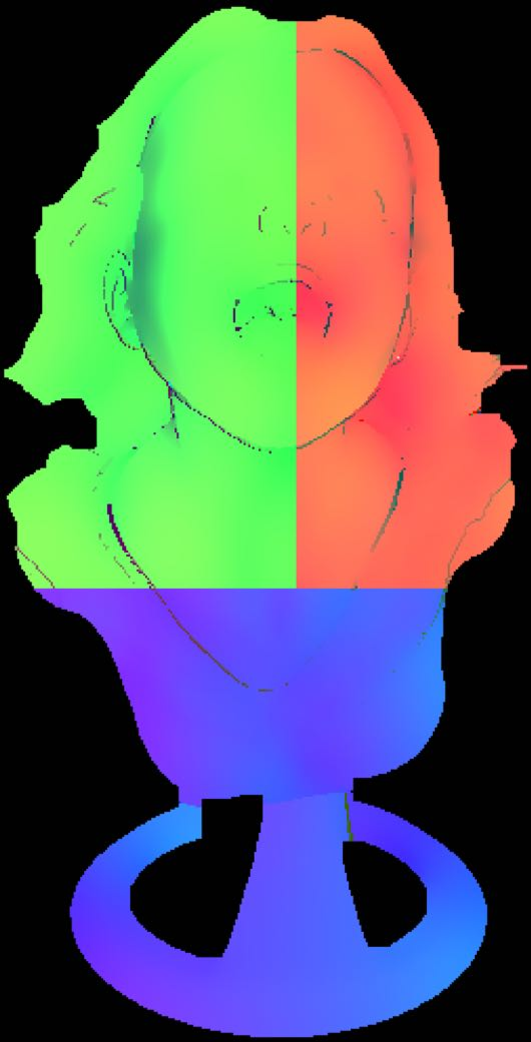
\includegraphics[height=0.25\linewidth]{figures/result/comp_fusion_rgb_albedo.pdf} &
  % Ours - SH2
 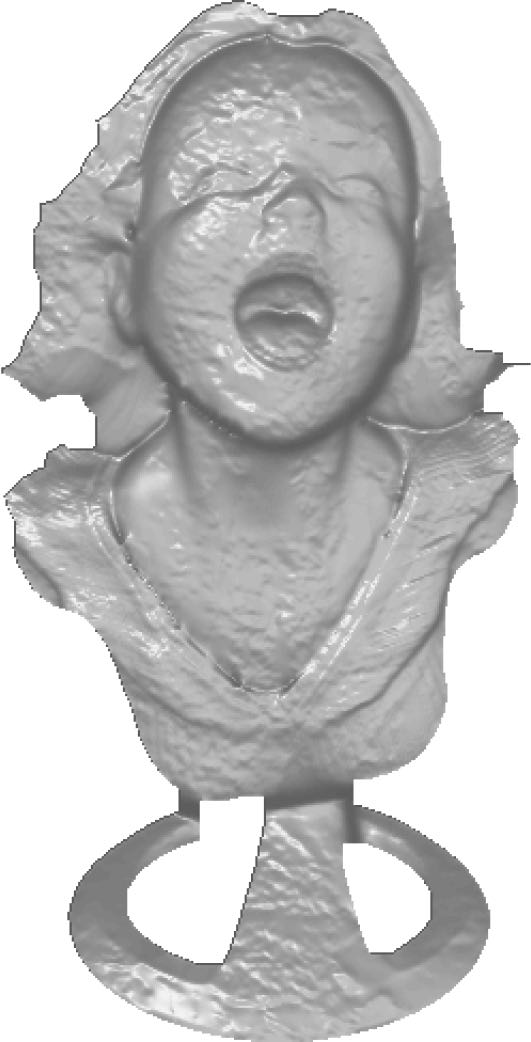
\includegraphics[height=0.25\linewidth]{figures/result/comp_fusion_pattern_shape.pdf} 
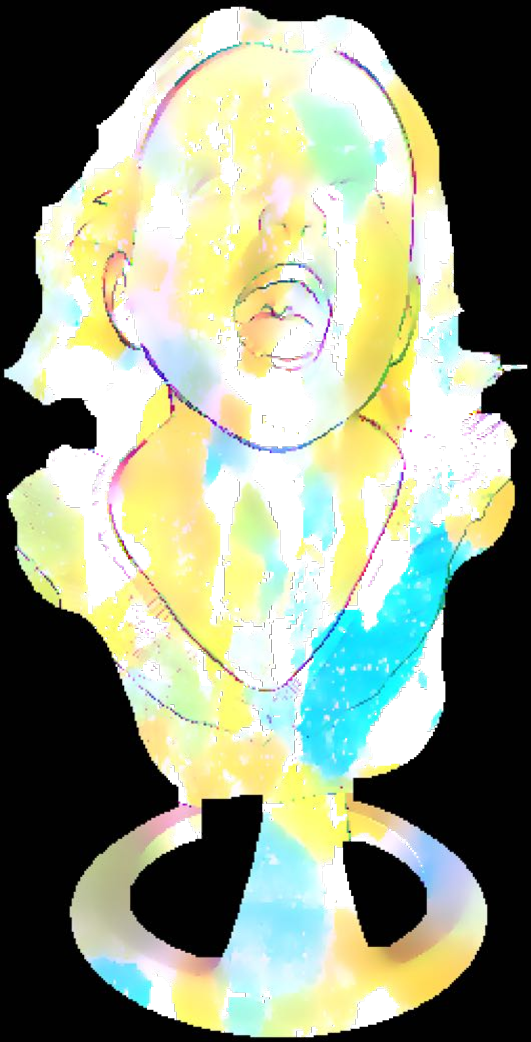
\includegraphics[height=0.25\linewidth]{figures/result/comp_fusion_pattern_albedo.pdf} &
  % Ours - SH2 color
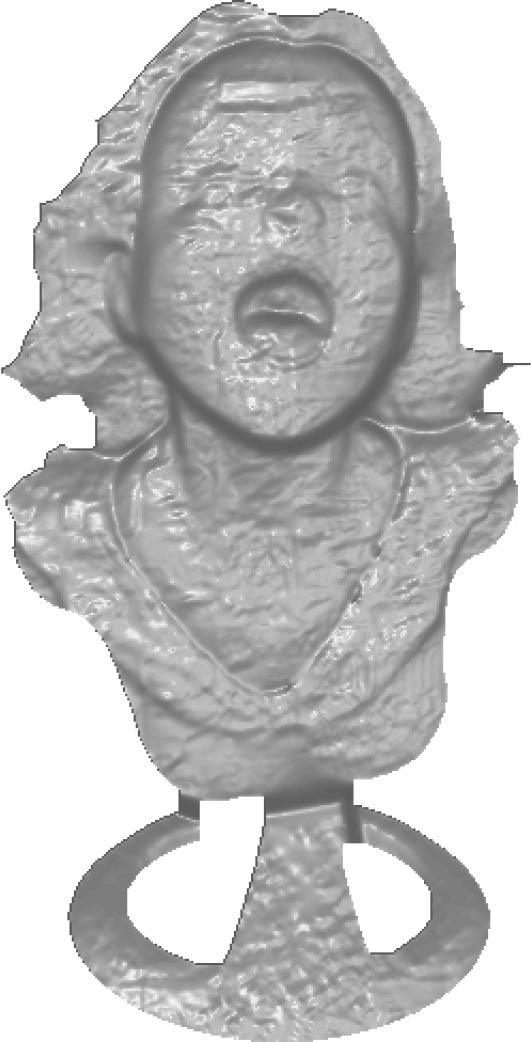
\includegraphics[height=0.25\linewidth]{figures/result/comp_fusion_love_shape.pdf} 
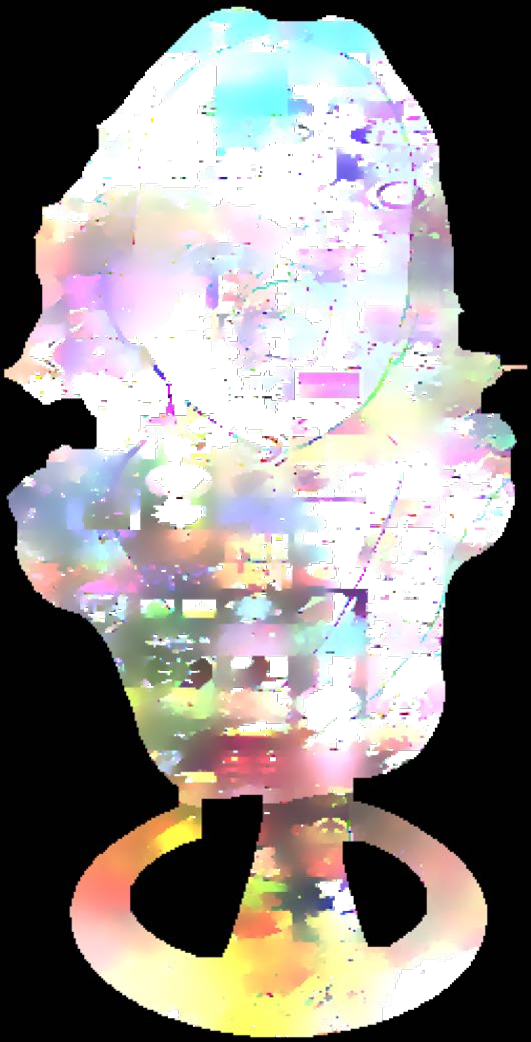
\includegraphics[height=0.25\linewidth]{figures/result/comp_fusion_love_albedo.pdf} \\
& {\small RMSE $= 2.87$, MAE $=17.17$} & {\small RMSE $= 2.88$, MAE $=17.73$} & {\small RMSE $=2.89$, MAE $=19.64$} \\
%%%%%%%%%%%%%%%%%%%%%%%%%%%%%%%%%%%%%%%%%%%%%%%%%%%%
% \multirow{2}{*}{
% \begin{tabular}{c}
%  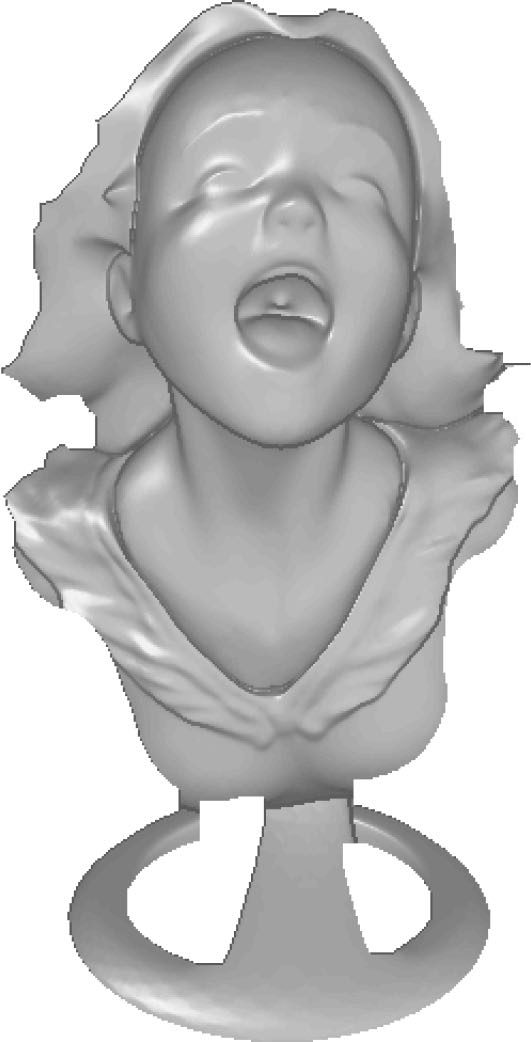
\includegraphics[width=0.1\linewidth]{figures/result/comp_input_shape.pdf} \\
%  Realistic \\
%   initialization \end{tabular}} &
    % Ours - Dir
\multirow{-15}{*}{\parbox[t]{2.5mm}{\rotatebox[origin=c]{90}{\small RGB Ratio}}} &    
 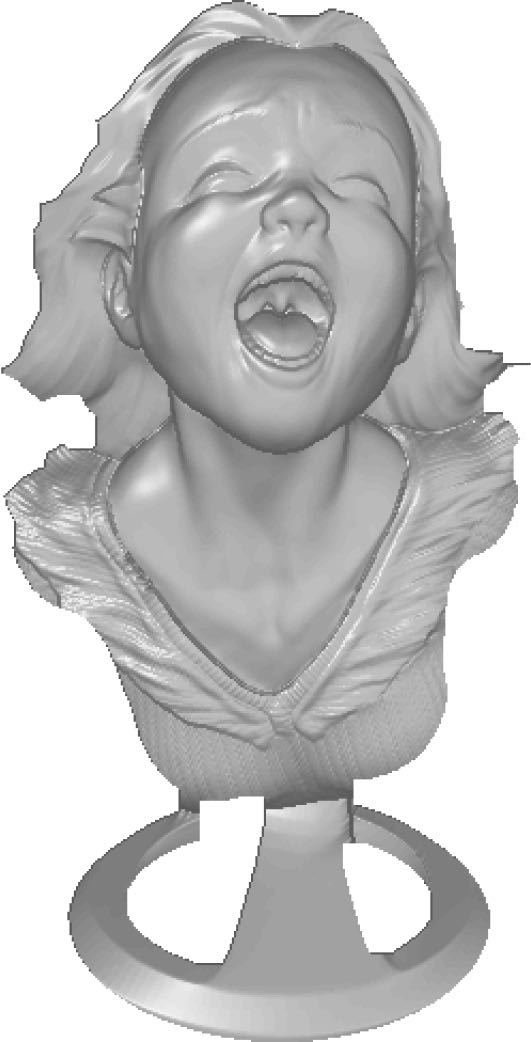
\includegraphics[height=0.25\linewidth]{figures/result/comp_ratio_rgb_shape.pdf}
 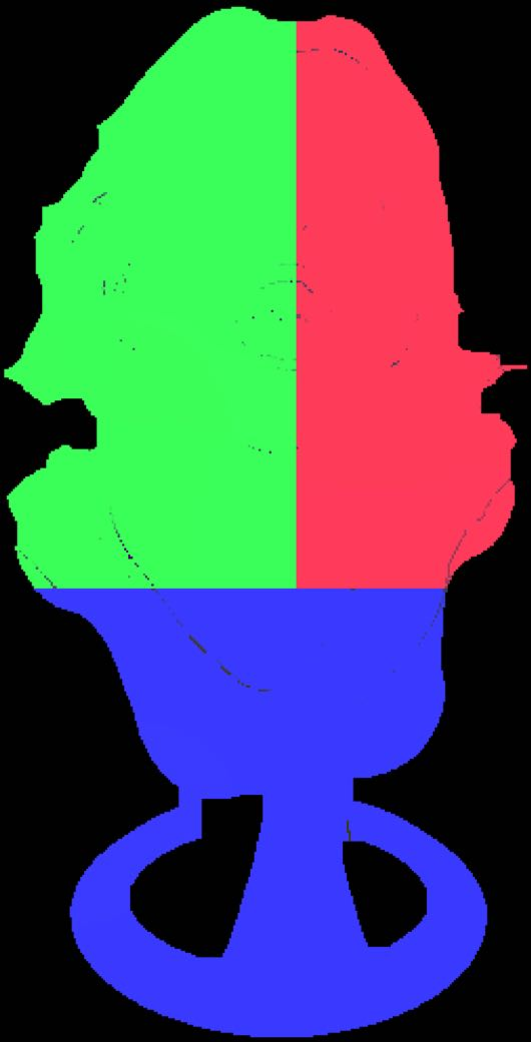
\includegraphics[height=0.25\linewidth]{figures/result/comp_ratio_rgb_albedo.pdf} &
  % Pattern
 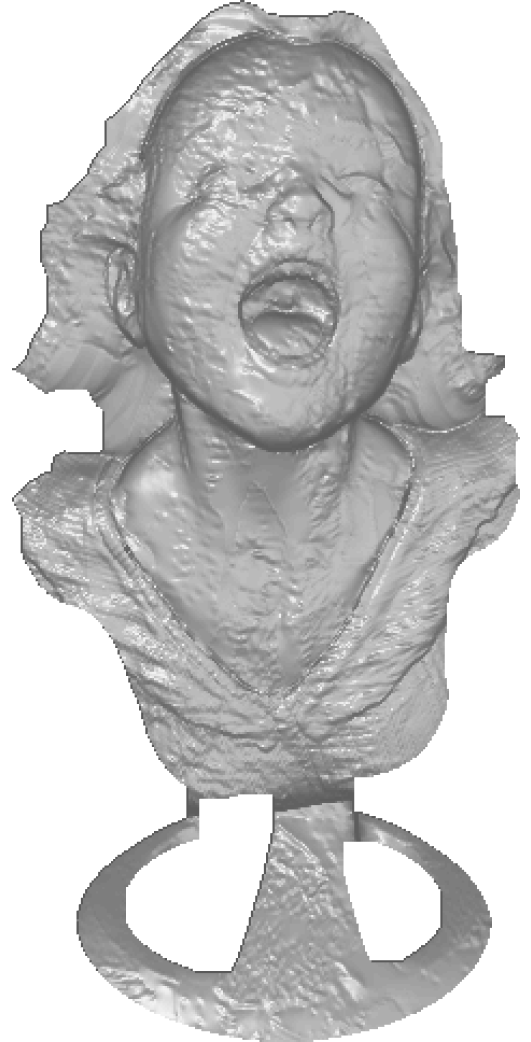
\includegraphics[height=0.25\linewidth]{figures/result/comp_ratio_pattern_shape.pdf} 
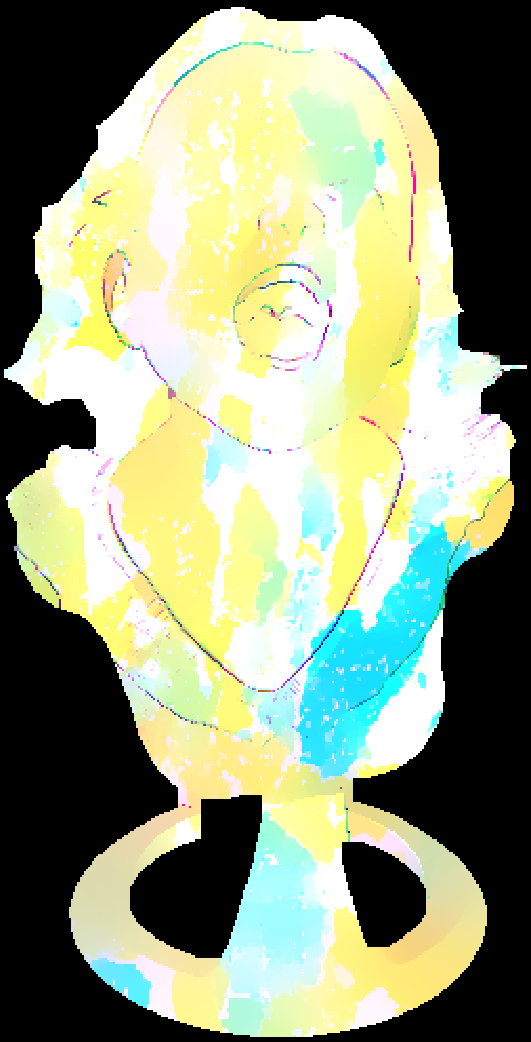
\includegraphics[height=0.25\linewidth]{figures/result/comp_ratio_pattern_albedo.pdf} &
  % Complicate Pattern
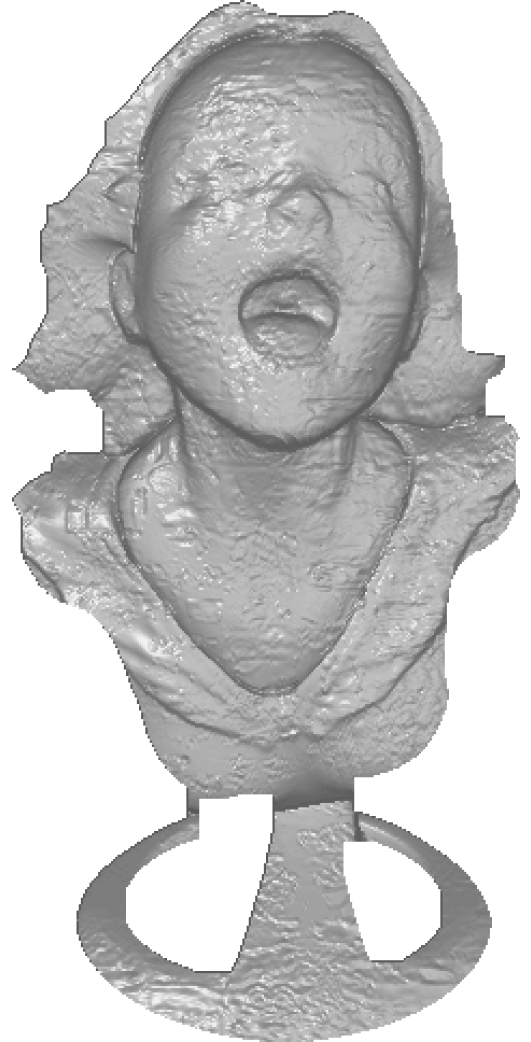
\includegraphics[height=0.25\linewidth]{figures/result/comp_ratio_love_shape.pdf} 
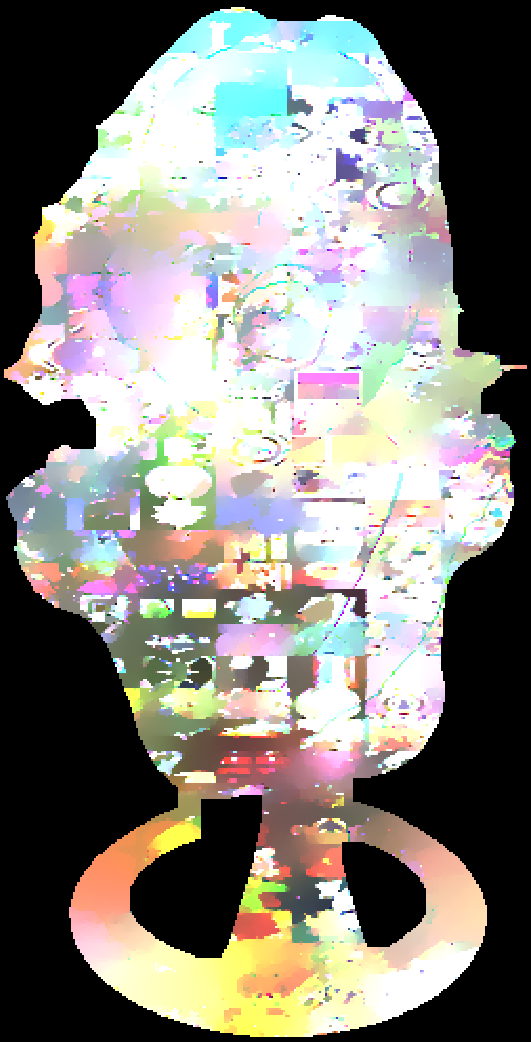
\includegraphics[height=0.25\linewidth]{figures/result/comp_ratio_love_albedo.pdf} \\
& {\small RMSE $= \textbf{1.94}$, MAE $=\textbf{5.06}$} & {\small RMSE $= 2.91$, MAE $=17.52$} & {\small RMSE $= 3.10$, MAE $=21.22$} \\
%%%%%%%%%%%%%%%%%%
  % Same for SIRFS
  % Ours - Dir
\multirow{-15}{*}{\parbox[t]{2.5mm}{\rotatebox[origin=c]{90}{\small Multi-Light}}} &   
 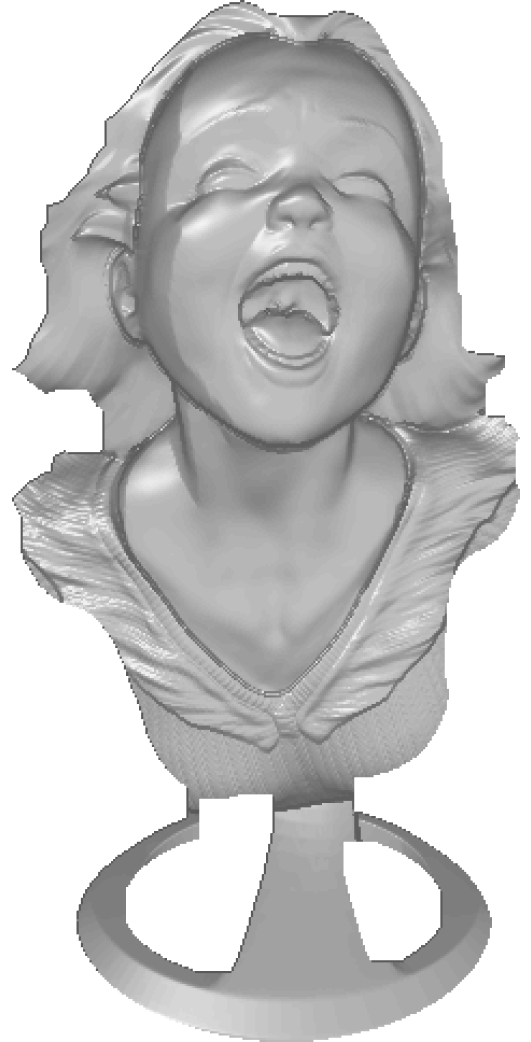
\includegraphics[height=0.25\linewidth]{figures/result/comp_robust_rgb_shape.pdf}
 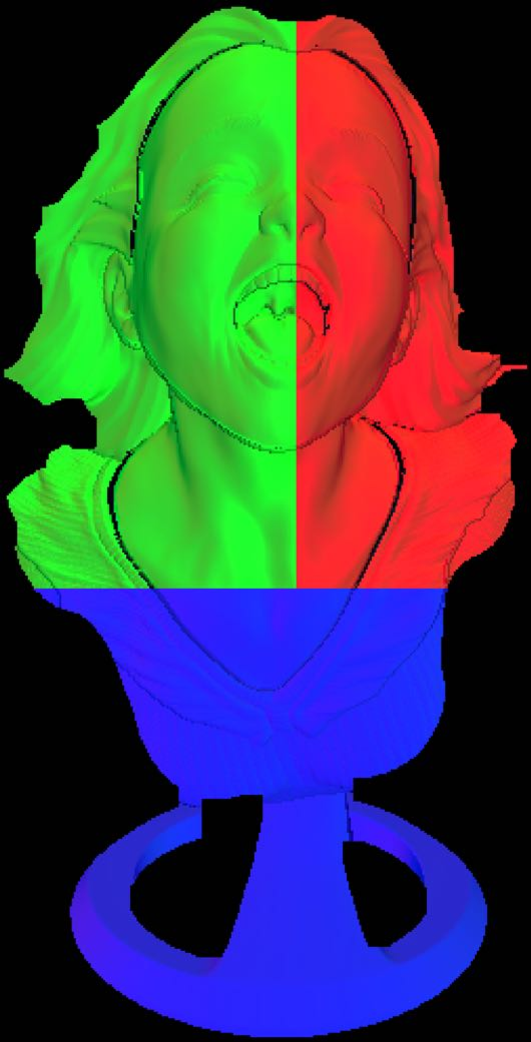
\includegraphics[height=0.25\linewidth]{figures/result/comp_robust_rgb_albedo.pdf} &
  % Pattern
 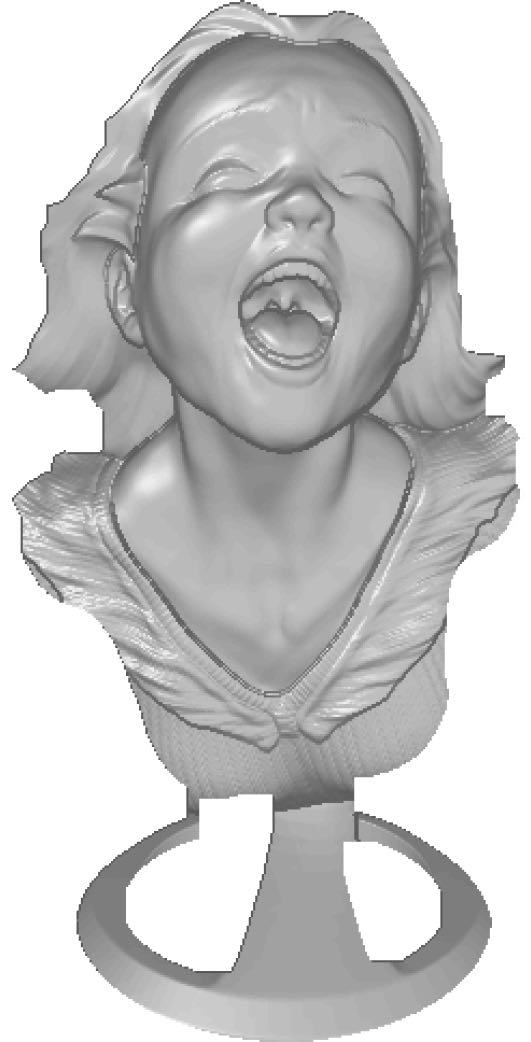
\includegraphics[height=0.25\linewidth]{figures/result/comp_robust_pattern_shape.pdf} 
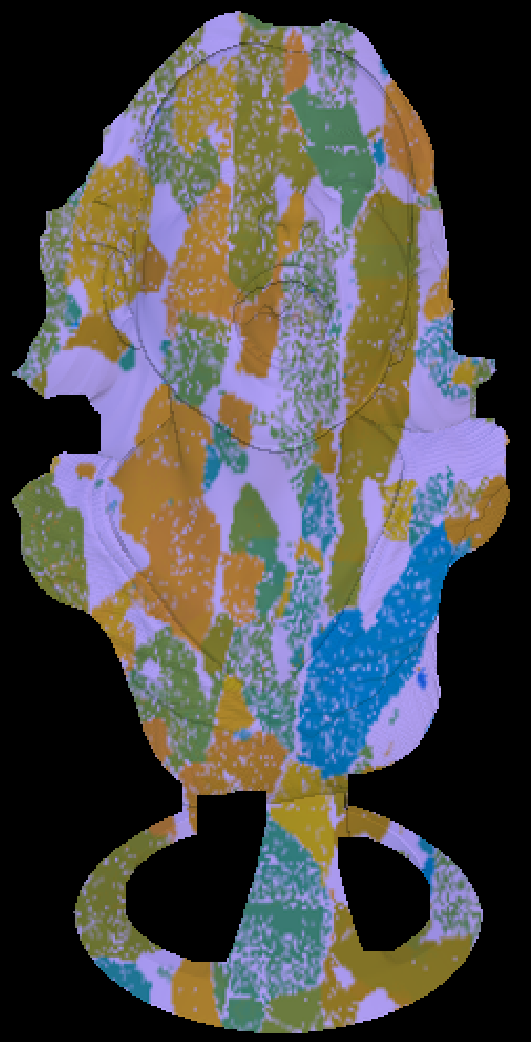
\includegraphics[height=0.25\linewidth]{figures/result/comp_robust_pattern_albedo.pdf} &
  % Complicate Pattern
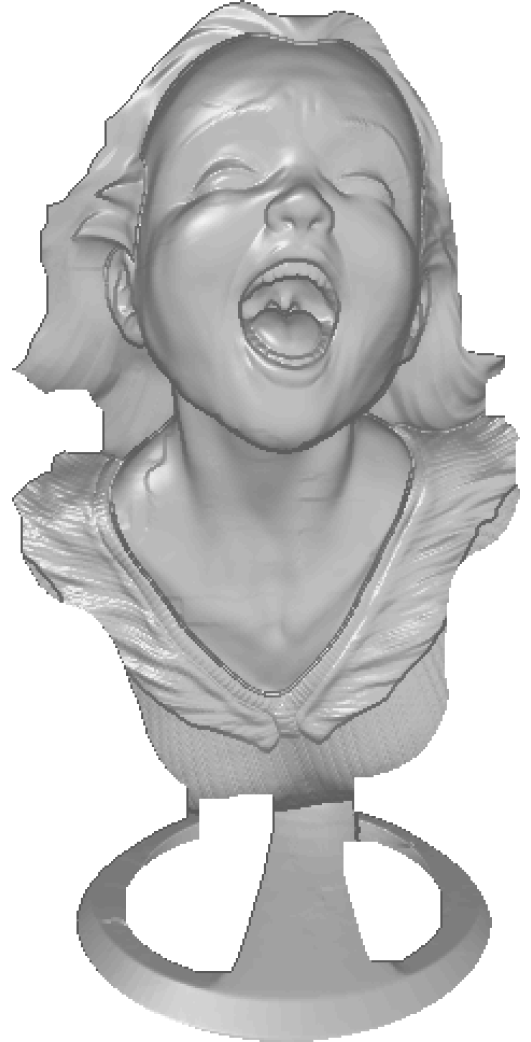
\includegraphics[height=0.25\linewidth]{figures/result/comp_robust_love_shape.pdf} 
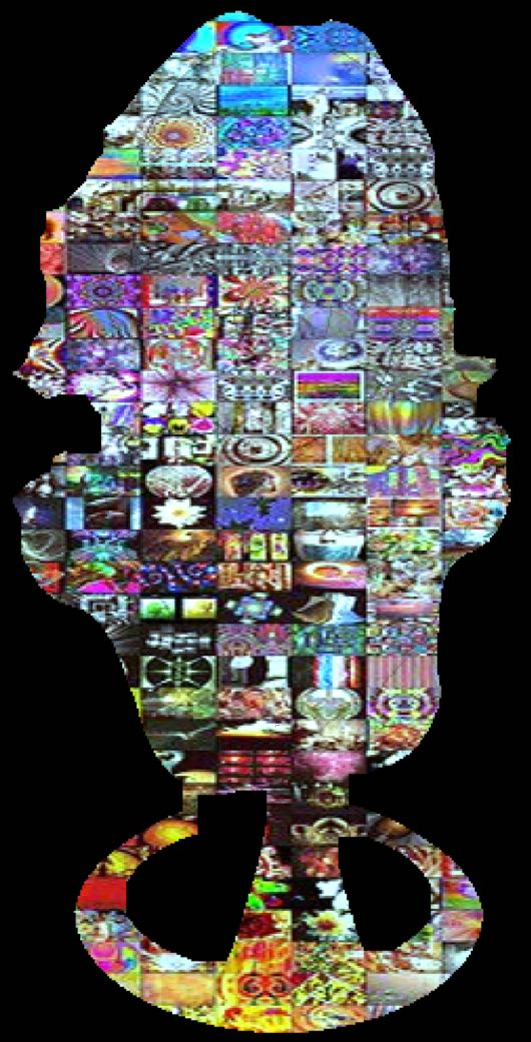
\includegraphics[height=0.25\linewidth]{figures/result/comp_robust_love_albedo.pdf} \\
& {\small RMSE $= 3.40$, MAE $=6.66$} & {\small RMSE $= \textbf{1.58}$, MAE $=\textbf{1.73}$} & {\small RMSE $= \textbf{1.84}$, MAE $=\textbf{2.68}$} \\
 \\
%%%%%%%%%%%%%%%%%%%%%%%%%%%%%%%%%%%%%%%%%%%%%%%%%%%%
  \end{tabular}
  }
  \caption{Evaluation of our two proposed methods RGB ratio and Robust Multi-Light method against our implementaion of RGBD-Fusion~\cite{or2015rgbd}, in three different albedos from simple to complicated. Our proposed methods outperform RGBD-Fusion in all tests with respect to both RMSE and MAE. The reference errors of input are 3.35 for RMSE and 16.75 for MAE.}
  \label{fig:result_syn_comp}
\end{figure}


%%%%%%%%%%%%%%%%%%%%%%%%%%%%%%%%%%%%%%%%%%%%
\section{Real Data Evaluations}
%----------------------------------------------

try to add noise on some of the images in the synthetic dataset and check the effectiveness of our method for robust normal recovery
%----------------------------------------------
\subsection{Complicated albedo objects}
%----------------------------------------------

%&&&&&&&&&&&&&&&&&&&&&&&&&
\begin{figure}[!ht]
\centering
\setlength{\tabcolsep}{0.1em} % column spacing
 {\renewcommand{\arraystretch}{1.6}% row spacing
\begin{tabular}{c|c c}
   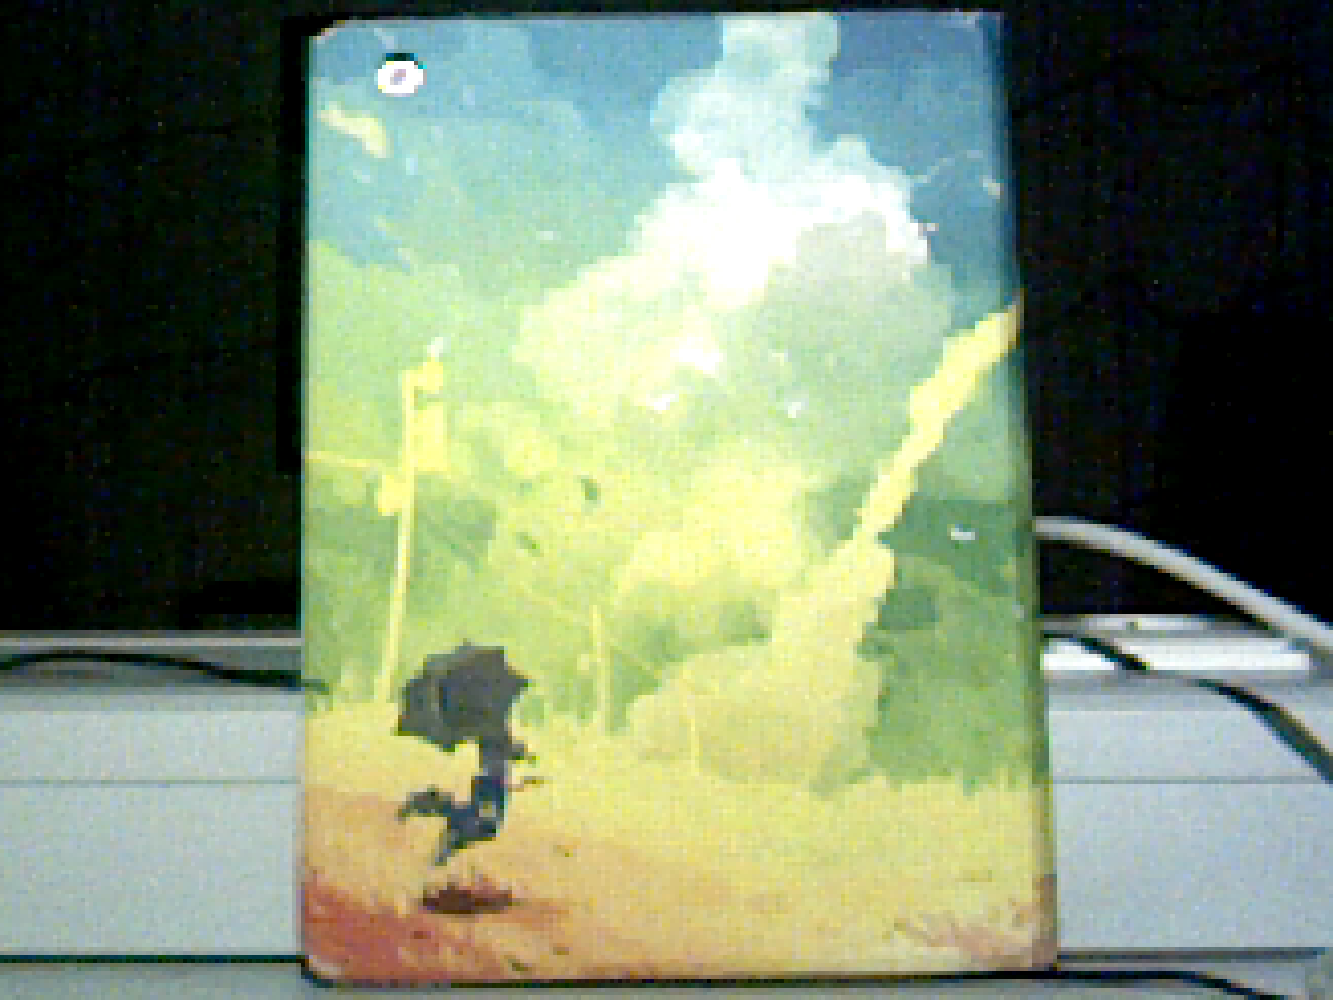
\includegraphics[height = 0.24\linewidth]{figures/result/robust_padback_rgb.pdf} 
   &
   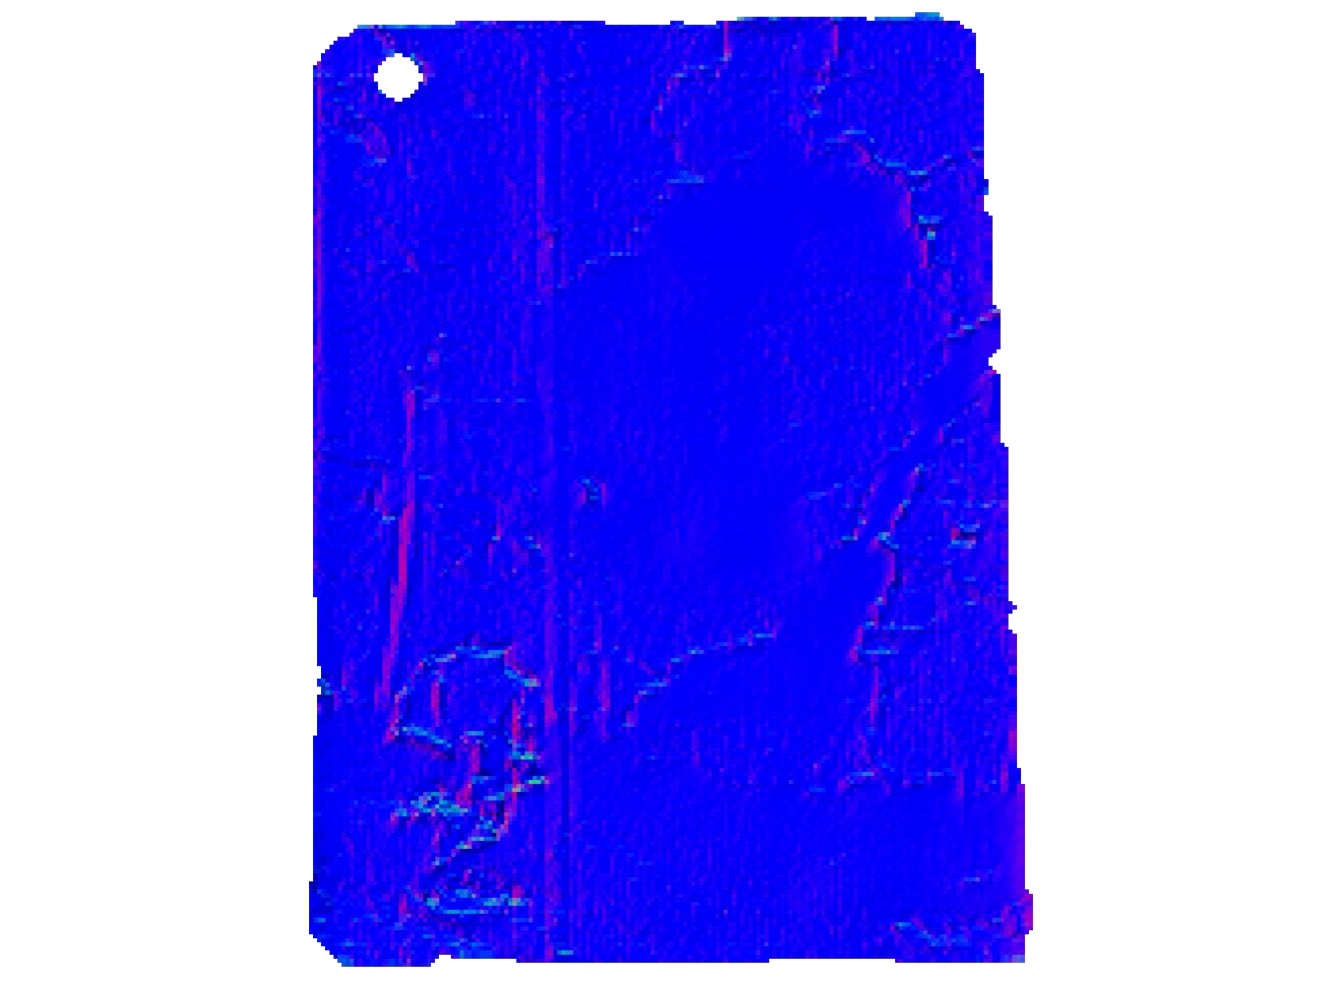
\includegraphics[height = 0.24\linewidth]{figures/result/rgbd_padback_normal.pdf} &
   \includegraphics[height = 0.24\linewidth]{figures/result/robust_padback_normal.pdf} \\

   \includegraphics[height = 0.24\linewidth]{figures/result/robust_padback_shape_init.pdf} 
   &
   \includegraphics[height = 0.24\linewidth]{figures/result/rgbd_padback_shape.pdf} &
   \includegraphics[height = 0.24\linewidth]{figures/result/robust_padback_shape.pdf}\\
\hline
   \includegraphics[height = 0.24\linewidth]{figures/result/robust_patternShirt_rgb.png} 
   &
   \includegraphics[height = 0.24\linewidth]{figures/result/rgbd_patternShirt_normal.png} &
   \includegraphics[height = 0.24\linewidth]{figures/result/robust_patternShirt_normal.png} \\

   \includegraphics[height = 0.24\linewidth]{figures/result/robust_patternShirt_shape_init.pdf} 
   &
   \includegraphics[height = 0.24\linewidth]{figures/result/rgbd_patternShirt_shape.pdf} &
   \includegraphics[height = 0.24\linewidth]{figures/result/robust_patternShirt_shape.pdf}\\


   {Input} & {RGBD-Fusion~\cite{or2015rgbd}} & {Proposed Multi-Light Model}               
 \end{tabular}}
\caption{Comparison our multi-light model with RGBD-Fusion in two specular objects. On the first column, the RGB images of the folder and the vase are ones of  the 10 various illuminations. First and third rows correspond to the surface normal from the refined depth, while second and fourth are the refined depth.}
\label{fig:comp_complicated_albedo}
\end{figure}
%&&&&&&&&&&&&&&&&&&&&&&&&&

%----------------------------------------------
\subsection{Specular (non-Lambertian) objects}
%----------------------------------------------


%&&&&&&&&&&&&&&&&&&&&&&&&&
\begin{figure}[!ht]
\centering
\setlength{\tabcolsep}{0.1em} % column spacing
 {\renewcommand{\arraystretch}{1.6}% row spacing
\begin{tabular}{c|c c}
   \includegraphics[height = 0.24\linewidth]{figures/result/robust_folder_rgb.pdf} 
   &
   \includegraphics[height = 0.24\linewidth]{figures/result/rgbd_folder_normal.pdf} &
   \includegraphics[height = 0.24\linewidth]{figures/result/robust_folder_normal.pdf} \\

   \includegraphics[height = 0.22\linewidth]{figures/result/robust_folder_shape_init.pdf} 
   &
   \includegraphics[height = 0.22\linewidth]{figures/result/rgbd_folder_shape.pdf} &
   \includegraphics[height = 0.22\linewidth]{figures/result/robust_folder_shape.pdf}\\
\hline
   \includegraphics[height = 0.24\linewidth]{figures/result/robust_vase_rgb.pdf} 
   &
   \includegraphics[height = 0.24\linewidth]{figures/result/rgbd_vase_normal.pdf} &
   \includegraphics[height = 0.24\linewidth]{figures/result/robust_vase_normal.pdf} \\

   \includegraphics[height = 0.24\linewidth]{figures/result/robust_vase_shape_init.pdf} 
   &
   \includegraphics[height = 0.24\linewidth]{figures/result/rgbd_vase_shape.pdf} &
   \includegraphics[height = 0.24\linewidth]{figures/result/robust_vase_shape.pdf}\\


   {Input} & {RGBD-Fusion~\cite{or2015rgbd}} & {Proposed Multi-Light Model}               
 \end{tabular}}
\caption{Comparison our multi-light model with RGBD-Fusion in two specular objects. On the first column, the RGB images of the folder and the vase are ones of  the 10 various illuminations. First and third rows correspond to the surface normal from the refined depth, while second and fourth are the refined depth.}
\label{fig:comp_complicated_albedo}
\end{figure}
%&&&&&&&&&&&&&&&&&&&&&&&&&



%%%%%%%%%%%%%%%%%%%%%%%%%%%%%%%%%%%%%%%%%%%%

